\section{Experimentacion y resultados}

Para analizar los algoritmos implementados vamos a utilizar varios archivos de test generados mediante Python como archivos de entrada, los cuales están más detallados en el apéndice, con el fin de realizar una serie de test que nos permitirán en primer caso encontrar parámetros buenos con lo que ejecutar los distintos métodos y posteriormente evaluar el desempeño de la implementación mediante las métricas propuestas por la cátedra.

Dividimos la experimentación en secciones, una para cada técnica. Y evaluaremos los parámetros individualmente para cada una de ellas

\subsection {Algoritmo de K-NN}

Lo primero que vamos a hacer es encontrar un valor de $K$ y la cantidad de vecinos más cercanos $k$ que nos permita maximizar la cantidad de aciertos, sin tener en consideración las métricas.

Ejecutamos el algoritmos de $K-NN$ variando los valores de k entre {1..30} dejando fija la cantidad de particiones para $K=$6 y $K=$15. Luego para cada una de las iteraciones tomamos el promedio. Esto se utilizó tanto para la cantidad de aciertos como para la cantidad de vecinos.

Cada uno de los conjuntos conto con 4200 imágenes a testear. En los siguientes gráficos presentamos algunos de los sets obtenidos:

Expresamos los aciertos para cada K en con el siguiente gráfico:
\begin{center}
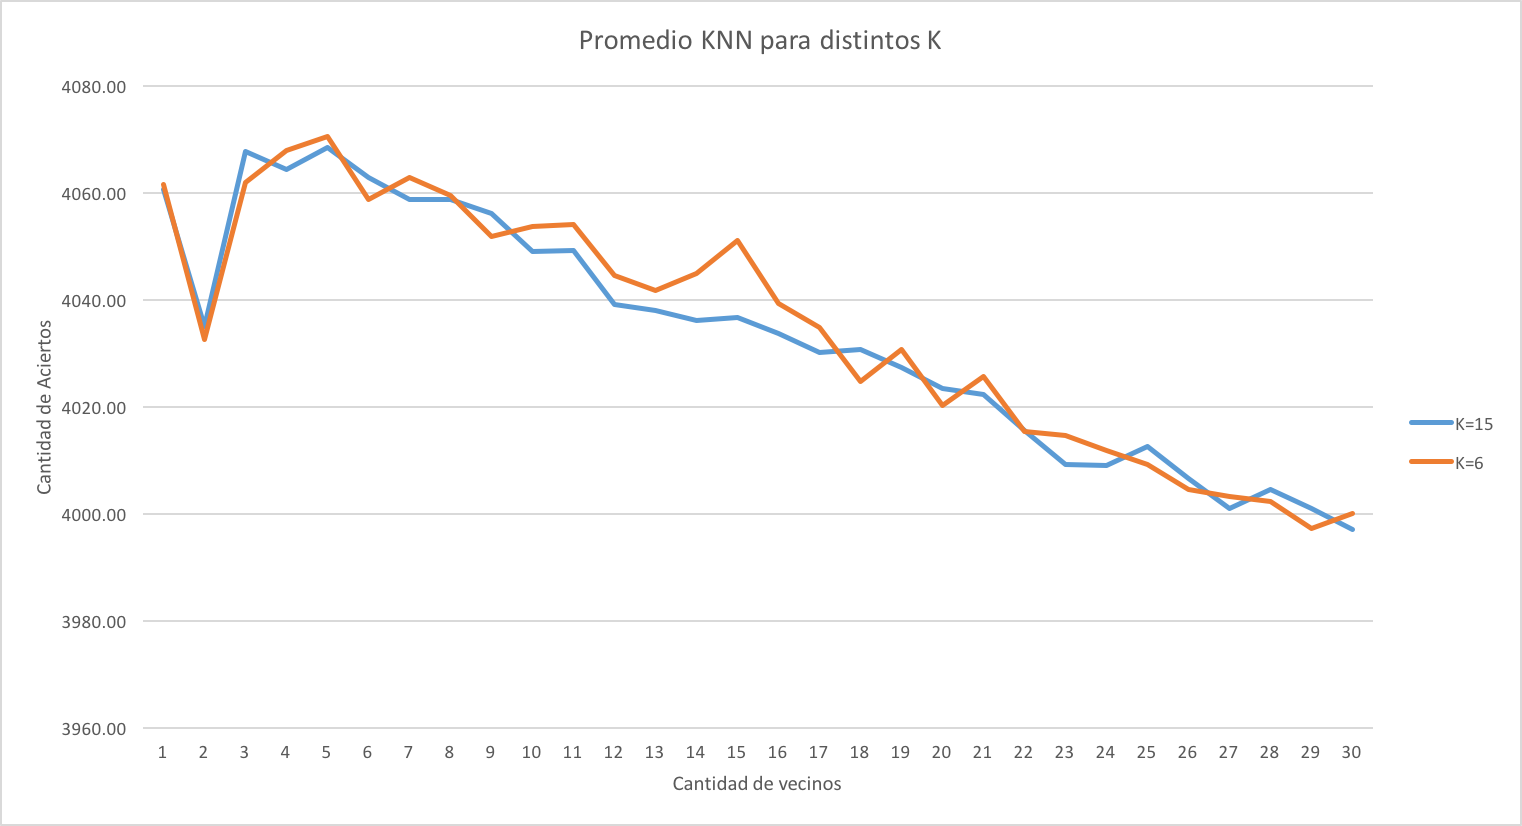
\includegraphics[scale=0.6]{imagenes/AciertosKNN.png}
\end{center}

Como se puede observar para para ambos $K$ se tiene el mismo patrón a lo largo que se incrementa la cantidad de vecinos $k$, pero ambas parecen alcanzar un máximo en $k=5$ como cantidad de vecinos. Además notemos que a medida que se incrementa el valor de $k$ la cantidad de aciertos va disminuyendo levemente, cumpliendo lo mencionado en el desarrollo. Cuanto más corta sea la distancia de los vecinos, más chances hay de tener un acierto sin importar el valor de $K$.

Si nos detenemos y observamos con más claridad cuando para la combinación de $K$=6 y $k$=5 es donde se maximizan en comparativa para knn, lo que intentaremos hacer en los próximos métodos es utilizar $K$=6 y ir variando la cantidad de vecinos más cercanos para ver si existe algún tipo de relación con el fin de asegurar que esa combinación es la mejor. Esto se debe a que no hay grandes diferencias entre las dos particiones que utilizamos, muy probablemente si el $K$ fuese mucho mayor la diferencia seria mayor.

Como segundo estudio, nos centramos en el análisis temporal para saber cómo afectaba la cantidad de particiones que tomamos para el Cross validation y variamos la cantidad de vecinos tomados para ver cómo se comportaba, los cuales arrojaron los siguientes resultados. 

\begin{center}
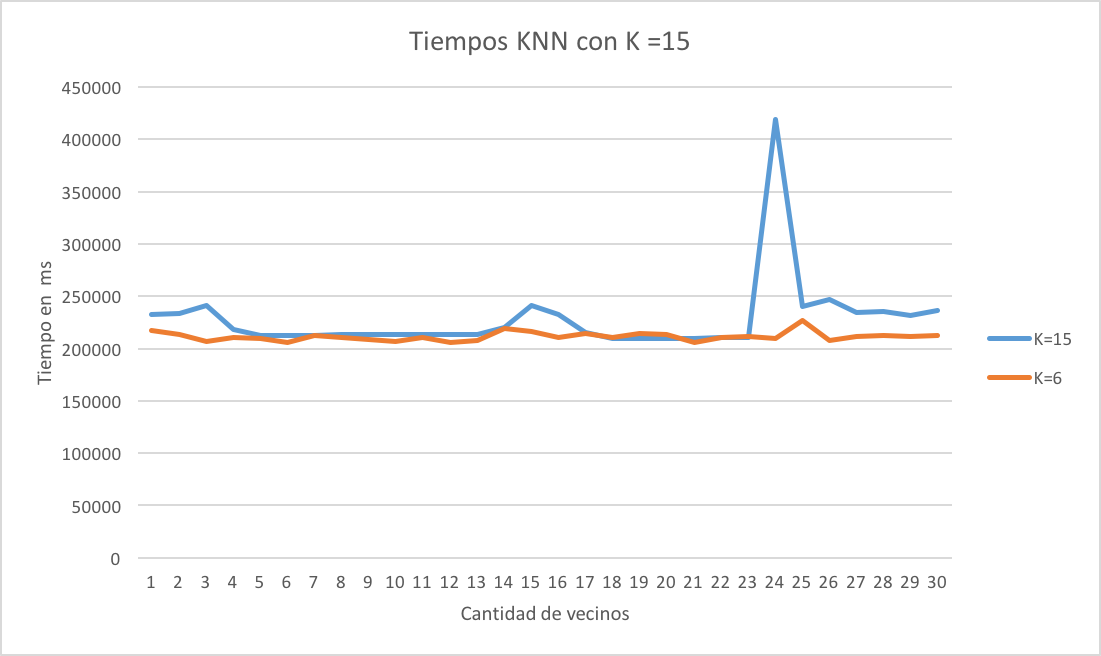
\includegraphics[scale=0.6]{imagenes/TiemposKNN.png}
\end{center}

En cuanto a los tiempos para diferentes $K$ no varían mucho en la media, si bien se puede notar al principio que a mayor cantidad de ejecuciones mayor es el tiempo que demora, algo previsible previamente.

Notemos  que hay un pico, o crecimiento repentino, cuando tomamos entre $k$=23 y $k$=25 vecinos más cercanos. Sin embargo, esto es un caso que deberíamos seguir ejecutando para esos parámetros con el fin de ver si no es ruido que se pudo haber generado por otro proceso en el momento de la ejecución para descartar esto.

\subsection {Algoritmo de K-NN con Optimización de PCA}

Para el algoritmo de PCA lo que realizamos fue una variación de los valores de lambda (cantidad de componentes principales). Para esos valores de $k$ medimos los tiempos de ejecución y los promediamos para poder ver de que manera varía la ejecución de los algoritmos en función de $\lamda$, luego tomamos un promedio de las ejecuciones y obtuvimos lo siguientes resultados:

\begin{center}
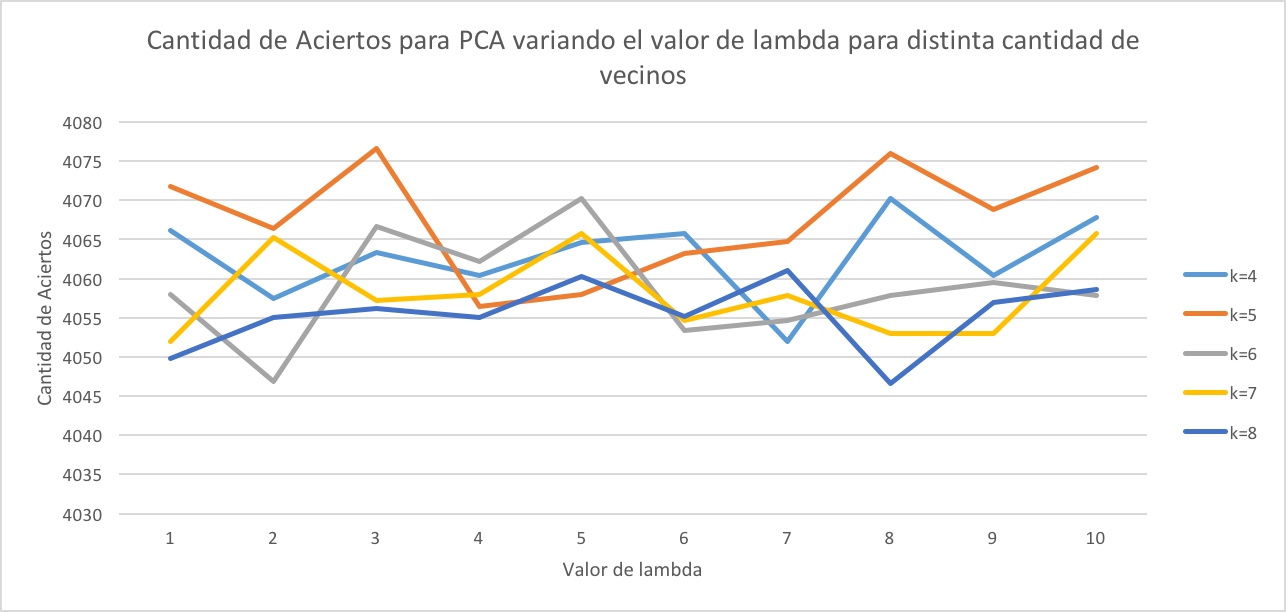
\includegraphics[scale=0.6]{imagenes/AciertosPCA.png}
\end{center}

Al ver estos resultados notamos a comparación de los resultados obtenidos para KNN con $k$=5 se respetan para la optimización, ya que mirando las combinaciones de lambda con cantidad de vecinos el que resulta como 'ganador' arrojando una cantidad de aciertos mayor a 4075 es cuando $k$=5 y $\lambda$=3. 

A medida crecía el lamda no parece llegar a igualarlo pero si está muy cerca cuando se toman 8 componentes principales. 

\begin{center}
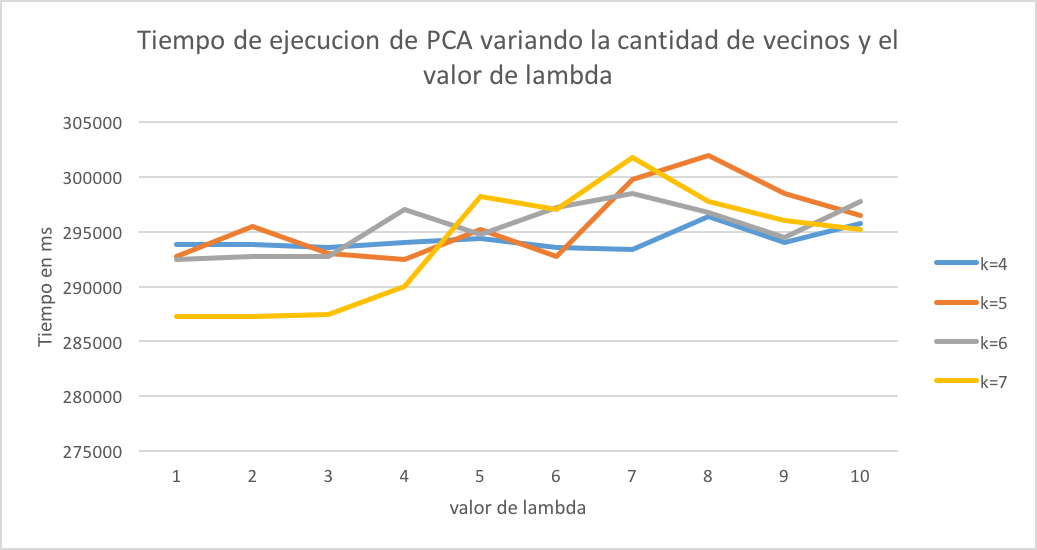
\includegraphics[scale=0.6]{imagenes/TiemposPCA.png}
\end{center}

En cuanto a los tiempos cabe aclarar que estos no contemplan todo lo que se considera el ’entrenamiento’ del sistema, es decir, todo el reprocesamiento que resultara en encontrar
los valores principales. La justificación de esto es que el procedimiento se realizar ́a una vez, para entrenar el sistema y luego, al momento de clasificar las
nuevas imágenes este tiempo podrá ser despreciado. Este grafico se puede ver que aumentar el α produce un aumento lineal de los tiempos de ejecución, 
de lo que se desprende que aumentar la cantidad valores principales no resulta gratuito en términos de tiempo de ejecución y tiene cierto costo asociado.

De igual manera la distribución de tiempos al variar el lamda parece ir creciendo levemente y podríamos predecir que así va a ser su comportamiento, mientras más grande sea el valor de lambda mayor tiempo va a consumir.

\subsection {Algoritmo de K-NN con Optimización de PSL-DA}

Para el algoritmo de PLS-DA hemos continuado con el mismo estudio para poder realizar una comparativa entre ambos en cuanto a su taza de acierto. Si observamos los resultados de PLSDA pretendemos observar resultados similares a PCA en cuanto a cantidad de aciertos. 

Luego de nuestros experimentos obtuvimos los siguientes resultados.

\begin{figure}[H]
\centering
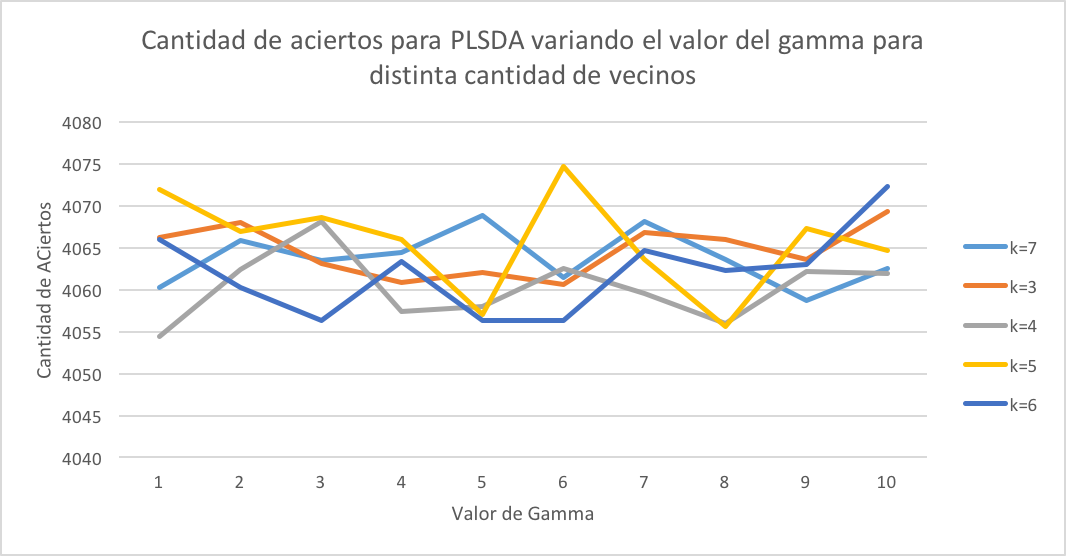
\includegraphics[width=1\textwidth]{imagenes/AciertosPLSDA.png}
\caption{Comparacion de aciertos variando el gamma}
\label{fig:Comparacion de tecnicas}
\end{figure}

De un modo muy parecido que para PCA con $\lambda$, podemos ver que si aumenta el $\gamma$, mejora la precisión pero si gamma aumenta demasiado , en algún momento empeora tu hit rate , suponemos que eso se debe a que si bien tenemos bastante información , la cantidad de vecinos no permite aprovecharla . Eso hace suponer que para que tengamos un buen hit rate , debe haber algún tipo de relación entre el $k$ y el $\gamma$.

En cuanto a los mejores valores para la ejecución de PLSDA, sigue sucediendo que utilizando $k$=5 es cuando se maximizan la taza de acierto. En este caso es mas grande la cantidad de componentes que utilizamos a la de $PCA$ y pero menor en cuanto a cantidad de aciertos. Esto puede deberse a que en la transformación estemos perdiendo calidad en los datos.

\begin{center}
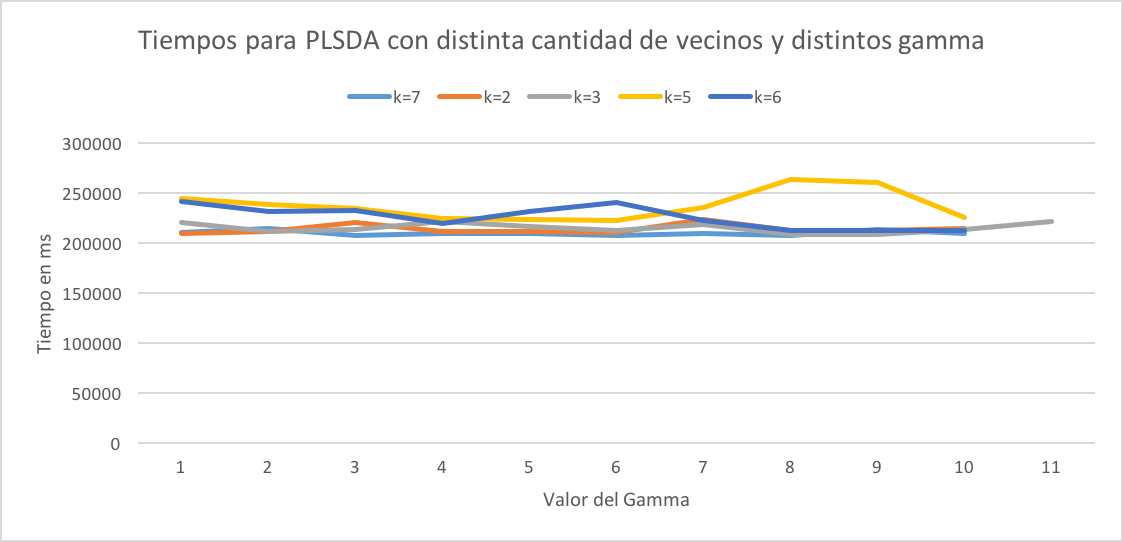
\includegraphics[scale=0.8]{imagenes/TiemposPLSDA.png}
\end{center}

Por otro lado tenemos diferencias en cuanto a el tiempo de ejecución entre PCA y PLSDA, el segundo parece ser un poco mas estable a la variación de componentes. A su vez es menor en cuanto a la de PCA, pero aquí es donde debemos analizar como podemos encontrar un balance en cuanto a tiempo de ejecución y cantidad de aciertos.

\subsection {Metricas Precision, Recall y F1 Score para los mejores resultados obtenidos}

El ultimo de los puntos pedidos con el fin de analizar la calidad de los resultados obtenidos era la utilización de 2 métricas de las presentadas en el enunciado. Para nuestros experimentos decidimos usar Precisión y Recall.

\textbf{Precisión} se basa en la cantidad de aciertos relativos dentro de una clase particular. Ósea, dada una clase $i$, definimos a los verdaderos positivos como $tp_i$ y los falsos positivos como $fp_i$, estos son aquellos que fueron definidos como una clase a la cual no pertenecían.
Con lo cual la precisión de dicha clase se define como 

tp_i / (tp_i + fp_i)

\textbf{Recall} es una medida para saber qué tan bueno es un clasificador para identificar a los que pertenecen a una clase, asumiendo que $fn_i$ son aquellos falsos negativos.
El Recall de una clase está definido como \\
tp_i / (tp_i + fn_i )

Luego para la mejor cantidad de vecinos obtenida (k=5); buscamos los valores de las métricas obtenidas para PCA.

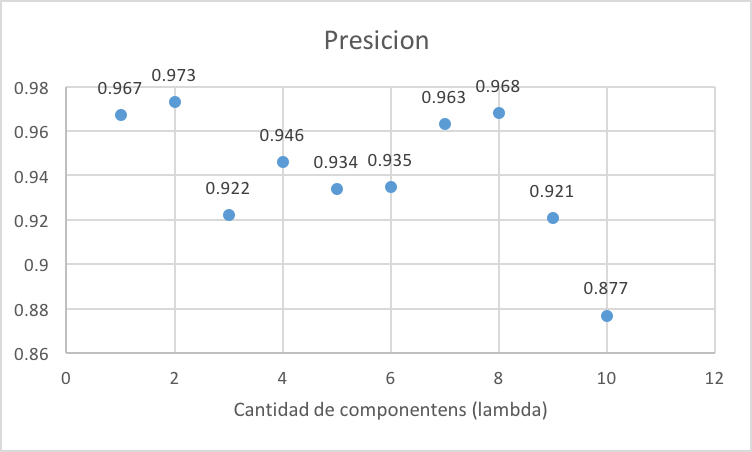
\includegraphics[scale=1]{imagenes/pcaPresicion.png}\\
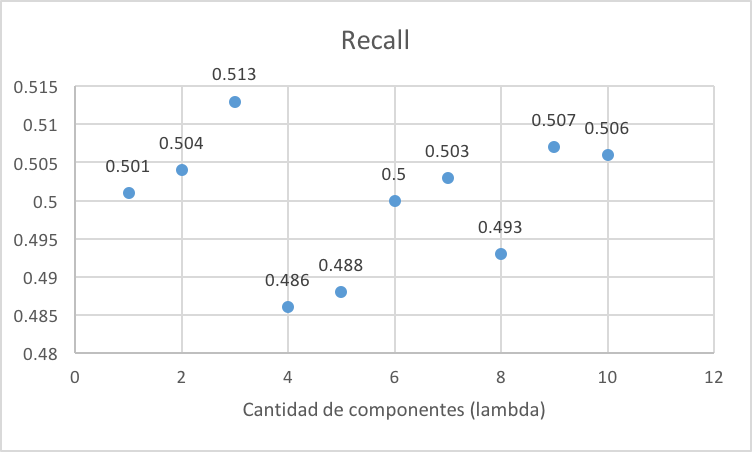
\includegraphics[scale=1]{imagenes/pcaRecall.png}

Como podemos ver los resultados para las métricas dieron muy parecidos en cuanto al lambda elegido para obtener el máximo dentro de la métrica. Sin embargo, esto está basado en que la cantidad de vecinos que tomamos es 5 dado a que en los experimentos de KNN+PCA demostrados con anterioridad fue con la cantidad de vecinos el cual obtuvimos los mejores resultados.

Por otro lado repetimos el análisis para PLSDA con el fin e analizar las mismas métricas y poder comparar

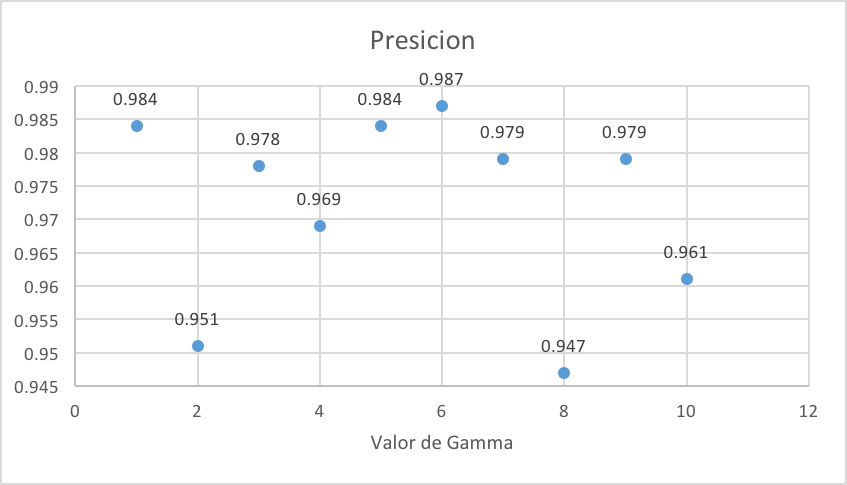
\includegraphics[scale=1]{imagenes/plsdaPresicion.png}\\
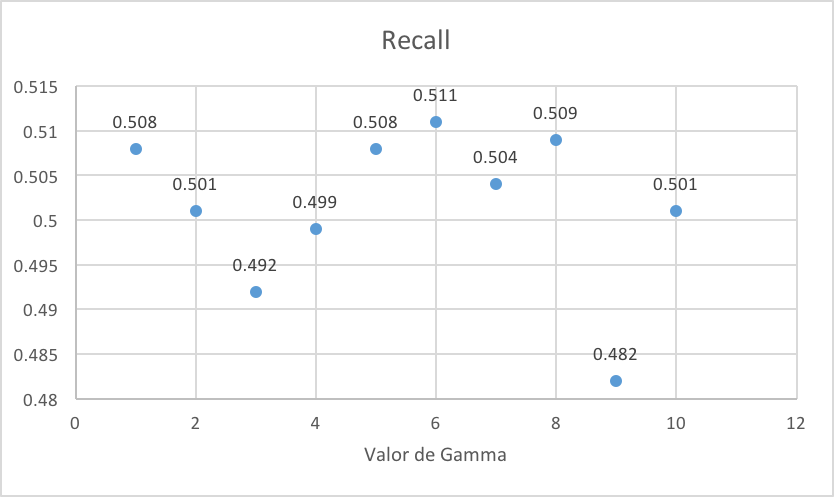
\includegraphics[scale=1]{imagenes/plsdaRecall.png}

En este caso podemos sacar la misma conclusión que en el caso anterior en cuanto a que las métricas para la combinación de $\gamma$ y $k$ con la cual se maximiza es la misma que para la cantidad de aciertos probados en los apartados anteriores.

Al momento de comparar basandonos en estos resultados podemos notar que $PLS-DA$ parece ser mas parejo en cuanto a la presicion, pero todo depende de los parametros elegidos. De igual manera en general parece no haber muchas diferencias entre ambos metodos, a excepcion del costo temporal de los algoritmos.

Por lo que podemos definir como que las mejores combinaciones de parámetros para $PCA$ y $PLS-DA$ son las dadas en este apartado. 
